%====================================================
%	CHAPTER 5 - Allocation
%====================================================
\chapter{Controller Allocation}
\label{ch:allocation}
%====================================================
The higher level attitude and position controllers (Sec:\ref{sec:control.attitude} and Sec:\ref{sec:control.position} respectively) design a desired virtual control input; $H(\vec{\mathbf{x}}_e,t)=\vec{\nu}_d=[\vec{F}_d~\vec{\tau}_d]^T$. The system's over-actuation was previously described in Sec:\ref{sec:control.inputs}; this chapter aims to solve for explicit actuator positions from that virtual input. Fig:\ref{fig:allocation-block} shows a simplified allocation block, reduced from Fig:\ref{fig:control-block}.
\begin{figure}[htbp]
\vspace{-8pt}
\centering
\begin{subfigure}{0.49\textwidth}
\centering
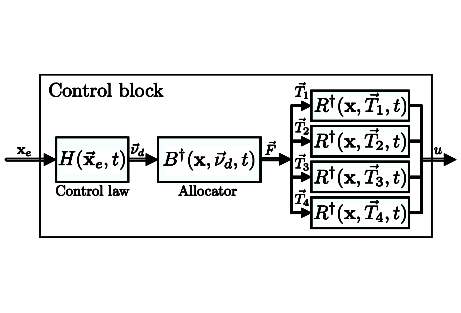
\includegraphics[width=\textwidth]{figs/allocator-block}
\caption{Allocation block}
\label{fig:allocation-block}
\end{subfigure}
\begin{subfigure}{0.49\textwidth}
\centering
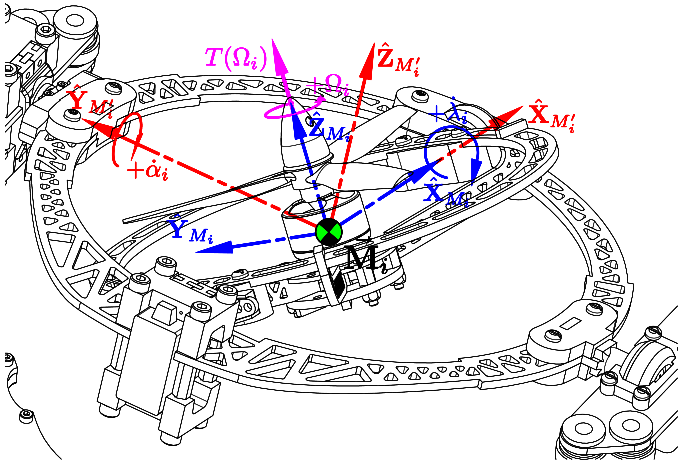
\includegraphics[width=\textwidth]{figs/force-redirect}
\caption{Single thrust vector construction}
\label{fig:allocation-redirect}
\end{subfigure}
\vspace{-10pt}
\caption{Actuator allocation}
\vspace{-16pt}
\end{figure}
\par
A distribution rule is needed to \emph{allocate} for physical actuator positions, $u_c\in\mathbb{U}$, to command that input $\vec{\nu}_c$, from Eq:\ref{eq:control-input}. Reiterating that (pseudo) inversion based allocation requires an affine actuator effectiveness function. The allocator is abstracted to first solve for four thrust vectors which are applied by each motor module, Eq:\ref{eq:4.7}.
\begin{equation}
B^{\dagger}(\mathbf{x},t)\vec{\nu}_d=\big[\vec{T}_1,~\vec{T}_2,~\vec{T}_3,~\vec{T}_4\big]^T
\end{equation}
Thereafter each 3D thrust vector is used to solve for each module's propeller's rotational speed and both servo rotational positions; effectively reversing the rotation applied by the structure in Fig:\ref{fig:allocation-redirect}.
\begin{equation}
[\Omega_i,~\lambda_i,~\alpha_i]^T=R^\dagger(\mathbf{x},\vec{T}_i,t)~~~~\text{for}~i\in[1:4]
\end{equation}
%====================================================
\section{Generalized allocation}
\label{sec:allocation.slack}
%====================================================
For regular, unconstrained control allocation the solution is posed as an optimization problem;\cite{allocation,controlallocation}. The objective is to minimize deviation between the virtual and commanded control inputs, $\vec{\nu}_d$ and $\vec{\nu}_c$ respectively. For some state control law's virtual input $\vec{\nu}_d=H(\vec{\mathbf{x}}_e,t)$:
\begin{equation}\label{eq:allocation-slack}
\underset{u\in\mathbb{U}^{m},~s\in\mathbb{R}^{n}}{min}\big(\norm{Q_s}\big)~~\text{such that}~~\vec{\nu}_d-\vec{\nu}_c=H(\vec{\mathbf{x}}_e,t)-B(\vec{\mathbf{x}},t,u)\triangleq s
\end{equation}
Where $u\in\mathbb{U}^m$ is the dimension of the actuator set and $(\vec{\mathbf{x}},~\vec{\nu}_d,~\vec{\nu}_c,~s)\in\mathbb{R}^{n}$ is the dimension of virtual plant inputs; specifically $n$ is the degrees of freedom the system has. In this case $u\in\mathbb{U}^{12}$ for 12 actuators and $\vec{\mathbf{x}}\in\mathbb{R}^6$ for the 6-DOF rigid body.
\par
In Eq:\ref{eq:allocation-slack}, $Q_s$ is some cost function to prioritize the slack variable, $s$, requirements. Typically that cost will just be the $L_2$ norm of the slack. Over-actuation means there exists an entire family of suitable actuator positions $u$ which are all solutions to Eq:\ref{eq:allocation-slack}. Solving for explicit actuator positions requires introduction of a secondary cost function, or control objective  $J(\vec{\mathbf{x}},t,u)$, into Eq:\ref{eq:allocation-slack}.
\begin{equation}\label{eq:allocation-problem}
\underset{u\in\mathbb{U}^{12},~s\in\mathbb{R}^{6}}{min}\big(||Q_s||+J(\vec{\mathbf{x}},u,t)\big)~~\text{such that}~~H(\vec{\mathbf{x}}_e,t)-B(\vec{\mathbf{x}},u,t)=s
\end{equation}
That secondary control objective $J(\vec{\mathbf{x}},t,u)$ and its associated \emph{explicit} solution to Eq:\ref{eq:allocation-problem} is the subject of control allocation research. Not much work has been done on over-allocation for aerospace vehicles outside the field of satellite attitude control (Section:\ref{subsubsec:intro.lit.control.allocation} for examples). Often satellites are over actuated for the sake of fault tolerance and redundancy\cite{FTCallocation,discreteFTC}. Actuator rate constraints can be further introduced such that $u$ is limited by $\Delta u$, constraining sequential actuator position changes.
\begin{multline}
\therefore\underset{u\in\mathbb{U}^{12},~s\in\mathbb{R}^6}{min}\big(||Q_s||+J(\vec{\mathbf{x}},u,t)\big)~~\text{s.t}~~H(\vec{\mathbf{x}}_e,t)-B(\vec{\mathbf{x}},u,t)=s\\\text{subject to}~~u=u_{n-1}+\Delta u,~\Delta u\in\mathbb{C}
\end{multline}
Most control allocation paradigms assume a linear, multiplicative relationship with the effectiveness function, hence the abstraction layer which was introduced previously in Eq:\ref{eq:4.7}. The allocator effectiveness function, when abstracted to a linear matrix multiplication, reduces to:
\begin{equation}
\begin{bmatrix}
\vec{F}_d\\
\vec{\tau}_d
\end{bmatrix}={\nu}_d=H(\vec{\mathbf{x}}_e,t)\Longleftrightarrow B(\vec{\mathbf{x}},u,t)=B'(\vec{\mathbf{x}},t)u=\vec{\nu}_c=\begin{bmatrix}
\vec{F}_c(u)\\
\vec{\tau}_c(u)
\end{bmatrix}
\end{equation}
With $\vec{\nu}_d\text{~and~}\vec{\nu}_c\in\mathbb{R}^n,~u\in\mathbb{U}\in\mathbb{R}^m,~B\in\mathbb{R}^{m\times n}$. That assumption makes addressing the allocation conceptually simpler, accommodating the use of inversion based allocation laws (Sec:\ref{subsec:allocation.allocators.inverse},\ref{subsec:allocation.allocators.weightedinverse},\ref{subsec:allocation.allocators.norminverse}).
%====================================================
\section{Thrust vector inversion}
\label{sec:allocation.inversion}
%====================================================
The rotation "inversion" function, $R^\dagger(\mathbf{x},\vec{F}_i,t)$, to solve for physical actuator positions $(\Omega_i,\lambda_i,\alpha_i)$, is as yet undefined. Assuming for now there is some allocation rule that, from $\vec{\nu}_d$, designs well four decomposed stabilizing 3-dimensional thrust vectors $\vec{T}_{1\rightarrow 4}$ to be produced by each motor module. It then follows that each of those four thrust vectors relate to their individual associated actuator positions through a quaternion \emph{rotation}, not transformation:
\begin{subequations}
\begin{equation}\label{eq:quaternion-thrust-allocation}
\vec{T}_i= Q_{M_i}\otimes\vec{T}(\Omega_i)\otimes Q_{M_i}^*~~~~\in\mathcal{F}^b
\end{equation}
\vspace{-16pt}
\begin{equation}\label{eq:quaternion-thrust-allocation-expanded}
=Q_{z}(\sigma_i)Q_{y}(\alpha_i)Q_{x}(\lambda_i)\otimes \vec{T}(\Omega_i) \otimes Q_{x}^*(\lambda_i)Q_{y}^*(\alpha_i)Q_z^*(\sigma_i)
\end{equation}
Where each motor thrust vector, $\vec{T}(\Omega_i)$, is calculated using thrust coefficients Eq:\ref{eq:thrust-coefficient} from Fig:\ref{fig:coeffs-plot}.
\begin{equation}
\vec{T}(\Omega_i)=\begin{bmatrix}
0\\
0\\
T(\Omega_i)
\end{bmatrix}=\begin{bmatrix}
0\\
0\\
C_T(J)\rho \Omega_i^2 D^4
\end{bmatrix}~~~~\in\mathcal{F}^{M_i}
\end{equation}
\end{subequations}
The thrust $T(\Omega_i)$ is in the direction of the rotor shaft's axis of rotation, bound to $\hat{Z}_{M_i}$. Seeing that quaternion rotation (\emph{transformation}) operators change the reference frame whilst retaining the vector operand's magnitude, it follows that $T(\Omega_i)$, and by extension the propeller speed $\Omega_i$, can be found:
\begin{subequations}
\begin{equation}
|\vec{T}_i|=\sqrt{\norm{[T_x~T_y~T_z]}}=\sqrt{T_x^2+T_y^2+T_z^2}=|T(\Omega_i)|=|C_T(J)\rho\Omega_i^2D^4|
\end{equation}
\vspace{-14pt}
\begin{equation}
\rightarrow \Omega_i=\sqrt{\frac{|\vec{T}_i|}{C_T(J)\rho D^4}}=\sqrt{\frac{\sqrt{T_x^2+T_y^2+T_z^2}}{C_T(J)\rho D^4}}
\end{equation}
\end{subequations}
Then reversing (or \emph{undoing}) the transformation from motor module to body frame in Eq:\ref{eq:quaternion-thrust-allocation}:
\begin{subequations}
\begin{equation}
\vec{T}(\Omega_i)=Q_{z}^*(\sigma_i)Q_{y}^*(\alpha_i)Q_{x}^*(\lambda_i)\otimes \vec{T}_i \otimes Q_{x}(\lambda_i)Q_{y}(\alpha_i)Q_z(\sigma_i)~~~~\in\mathcal{F}^{M_i}
\end{equation}
\vspace{-14pt}
\begin{equation}
\rightarrow \vec{T}(\Omega_i)=Q_{M_i}^*\otimes \vec{T}_i \otimes Q_{M_i}~~~~\in\mathcal{F}^{M_i}
\end{equation}
\end{subequations}
Knowing only $\vec{T}(\Omega_i)$ and $\vec{T}_i$ in the motor frame and body frame respectively requires solving for a quaternion which relates the two. If both vectors are of unit length, $\hat{T}_i$ and $\hat{T}(\Omega_i)$; then the following relationship can be used to construct a relative quaternion:
\begin{subequations}
\begin{equation}
\hat{T}_i\triangleq\frac{\vec{T}_i}{|\vec{T}_i|}=\frac{\vec{T}_i}{\sqrt{T_x^2+T_y^2+T_z^2}}~~~~\in\mathcal{F}^b
\end{equation}
\vspace{-8pt}
\begin{equation}
\hat{T}(\Omega_i)\triangleq\frac{\vec{T}(\Omega_i)}{|\vec{T}(\Omega_i)|}=\frac{\vec{T}(\Omega_i)}{|C_T(J)\rho\Omega^2 D^4|}=\begin{bmatrix}
0 & 0 & 1
\end{bmatrix}^T~~~~\in\mathcal{F}^{M_i}
\end{equation}
\vspace{-4pt}
\begin{equation}\label{eq:vector-quaternion}
Q_{M_i}=\begin{bmatrix}
q_0\\
\vec{q}
\end{bmatrix}
=
\begin{bmatrix}
1+\hat{T}_i\cdot \hat{T}(\Omega_i)\\
-\hat{T}_i\times\hat{T}(\Omega_i)
\end{bmatrix}
\end{equation}
\end{subequations}
Where Eq:\ref{eq:vector-quaternion} is adapted from the inherent quaternion definition which rotates a vector around a single Euler axis, Eq:\ref{eq:quaternion-euler-axis}, when applied to two unit vectors. That quaternion can indeed be used to solve for relative pitch, roll and yaw Euler angles (Appendix:\ref{app:equations.quaternions}). The problem is that Eq:\ref{eq:vector-quaternion} solves for the \textbf{most direct, shortest path} rotation from one vector to another. In most cases, a sequenced Z-Y-X rotation is by no means the shortest rotational possible path. Solutions for $[\phi,\theta,\psi]^T$ from Eq:\ref{eq:vector-quaternion} are not useful for trying to resolve suitable servo positions $\lambda_i$ and $\alpha_i$.
\par
The associated $[\phi,~\theta,~\psi]^T$ solutions to Eq:\ref{eq:app-quaternion-eule} are then of no consequence in trying to solve for sequence of rotation angles $[\lambda_i,~\alpha_i,~\sigma_i]^T$, where $\sigma_i$ is already known to be an orthogonal multiplicate. Furthermore, when considering a sequenced Z-Y-X quaternion, no further insight can be extracted without applying very complicated trigonometric inversions:
\begin{subequations}
\begin{equation}
Q_b=\begin{bmatrix}
cos\frac{\psi}{2}\\
0\\
0\\
sin\frac{\psi}{2}
\end{bmatrix}
\otimes
\begin{bmatrix}
cos\frac{\theta}{2}\\
0\\
sin\frac{\theta}{2}\\
0
\end{bmatrix}
\otimes
\begin{bmatrix}
cos\frac{\phi}{2}\\
sin\frac{\phi}{2}\\
0\\
0
\end{bmatrix}
\end{equation}
\begin{equation}
=
\begin{bmatrix}
c\frac{\psi}{2}c\frac{\theta}{2}c\frac{\phi}{2}+s\frac{\psi}{2}s\frac{\theta}{2}s\frac{\phi}{2}\\
c\frac{\psi}{2}c\frac{\theta}{2}s\frac{\phi}{2}-s\frac{\psi}{2}s\frac{\theta}{2}c\frac{\phi}{2}\\
c\frac{\psi}{2}s\frac{\theta}{2}c\frac{\phi}{2}+s\frac{\psi}{2}c\frac{\theta}{2}s\frac{\phi}{2}\\
s\frac{\psi}{2}c\frac{\theta}{2}c\frac{\phi}{2}-c\frac{\psi}{2}s\frac{\theta}{2}s\frac{\phi}{2}
\end{bmatrix}
=
\begin{bmatrix}
q_0\\
q_x\\
q_y\\
q_z
\end{bmatrix}
=
\begin{bmatrix}
q_0\\
\vec{q}
\end{bmatrix}
\end{equation}
\begin{equation}
\rightarrow\vec{T}_i=
\begin{bmatrix}
c\frac{\psi}{2}c\frac{\theta}{2}c\frac{\phi}{2}+s\frac{\psi}{2}s\frac{\theta}{2}s\frac{\phi}{2}\\
c\frac{\psi}{2}c\frac{\theta}{2}s\frac{\phi}{2}-s\frac{\psi}{2}s\frac{\theta}{2}c\frac{\phi}{2}\\
c\frac{\psi}{2}s\frac{\theta}{2}c\frac{\phi}{2}+s\frac{\psi}{2}c\frac{\theta}{2}s\frac{\phi}{2}\\
s\frac{\psi}{2}c\frac{\theta}{2}c\frac{\phi}{2}-c\frac{\psi}{2}s\frac{\theta}{2}s\frac{\phi}{2}
\end{bmatrix}
\otimes
\vec{T}(\Omega_i)
\otimes
\begin{bmatrix}
s\frac{\psi}{2}s\frac{\theta}{2}s\frac{\phi}{2}+c\frac{\psi}{2}c\frac{\theta}{2}c\frac{\phi}{2}\\
s\frac{\psi}{2}s\frac{\theta}{2}c\frac{\phi}{2}-c\frac{\psi}{2}c\frac{\theta}{2}s\frac{\phi}{2}\\
-c\frac{\psi}{2}s\frac{\theta}{2}c\frac{\phi}{2}-s\frac{\psi}{2}c\frac{\theta}{2}s\frac{\phi}{2}\\
c\frac{\psi}{2}s\frac{\theta}{2}s\frac{\phi}{2}-s\frac{\psi}{2}c\frac{\theta}{2}c\frac{\phi}{2}
\end{bmatrix}
\end{equation}
\end{subequations}
Instead; returning to rotation matrices for the inverse transformation and reiterating that Euler angle equivalents for the servos are; $[\phi,~\theta,~\psi]^T\iff [\lambda_i,~\alpha_i,~\sigma_i]^T$. It then follows (where \emph{$i^{th}$ motor subscripts} $1\rightarrow 4$ are implied):
\begin{subequations}
\begin{equation}
\vec{T}_i=\begin{bmatrix}
c\sigma & -s\sigma & 0\\
s\sigma & c\sigma & 0\\
0 & 0 & 1 
\end{bmatrix}
\begin{bmatrix}
c\alpha & 0 & s\alpha\\
0 & 1 & 0\\
-s\alpha & 0 & c\alpha
\end{bmatrix}
\begin{bmatrix}
1 & 0 & 0\\
0 & c\lambda & -s\lambda\\
0 & s\lambda & c\lambda
\end{bmatrix}\vec{T}(\Omega_i)
\end{equation}
\begin{equation}
\rightarrow\vec{T}_i=\begin{bmatrix}
c\sigma c\alpha & c\sigma s\alpha s\lambda - s\sigma c\lambda & c\sigma s\alpha c\lambda + s\sigma s\lambda\\
s\sigma c\alpha & s\sigma s\alpha s\lambda + c\sigma c\lambda & s\sigma s\alpha c\lambda - c\sigma s\lambda\\
-s\alpha & c\alpha s\lambda & c\alpha c\lambda
\end{bmatrix}
\begin{bmatrix}
0\\
0\\
T(\Omega_i)
\end{bmatrix}
\end{equation}
\begin{equation}\label{eq:rotation-inverse}
\rightarrow
\begin{bmatrix}
T_x\\
T_y\\
T_z
\end{bmatrix}
=\begin{bmatrix}
s\sigma s\lambda + c\sigma s\alpha c\lambda\\
s\sigma s\alpha c\lambda - c\sigma s\alpha\\
c\alpha c\lambda
\end{bmatrix}
T(\Omega_i)
\end{equation}
\end{subequations}
Where $\sigma$ is an orthogonal multiple which rotates the vector about the $\hat{Z}_b$ axis. The fact that the principle thrust vector $\vec{T}(\Omega_i)$ has only a $\hat{Z}_{M_i}$ component in the motor frame makes the solution for servo angles dramatically less complex. Then Eq:\ref{eq:rotation-inverse} simplifies even further to the following four trigonometric relations respectively for each motor module:
\begin{equation}
\begin{bmatrix}
T_x\\
T_y\\
T_z
\end{bmatrix}
=
\begin{bmatrix}
\begin{bmatrix}
s\alpha c\lambda\\
-s\lambda \\
c\alpha c\lambda
\end{bmatrix}
,
\begin{bmatrix}
s\lambda\\
s\alpha c\lambda\\
c\alpha c\lambda
\end{bmatrix}
,
\begin{bmatrix}
-s\alpha c\lambda\\
s\lambda\\
c\alpha c\lambda
\end{bmatrix}
,
\begin{bmatrix}
-s\lambda\\
-s\alpha c\lambda\\
c\alpha c\lambda
\end{bmatrix}
\end{bmatrix}T(\Omega_i)~~~\text{for}~~i\in[1,~2,~3,~4]
\end{equation}
It then becomes a simple case of inverse trigonometry to solve for both $\lambda_i$ and $\alpha_i$. For the example case of $i=1$, the sequel holds true and can similarly be extended to the remaining modules. Firstly using $T(\Omega_i)=||\vec{T}_i||$ and implementing a four quadrant secondary arctangent2 function. Wherein $arctan2(x,y)$ is the four-quadrant tangent inverse\cite{atan2}, producing the principle argument of the complex operands:
\begin{equation}
arctan2(x,~y)=PR~arg(x+y\hat{i})=Arg(x+y\hat{i})
\end{equation}
The use of a full quadrature arctangent function is to find solutions for Euler angles that are not only acute. Then exploiting the fact that $arctan(x)\equiv arcsin(x/\sqrt{1-x^2})$:
\begin{subequations}
\begin{equation}
\lambda_i =  arctan2\bigg(-T_y,~\sqrt{||\vec{T}_i||^2-T_y^2}\hspace{2pt}\bigg)
\end{equation}
\vspace{-10pt}
\begin{equation}
\alpha_i = arctan2\big(T_x,~T_z\hspace{2pt}\big)
\end{equation}
\end{subequations}
Therefore, the secondary component of the control allocation block, $R^\dagger(\mathbf{x},\vec{T}_i,t)$ from Fig:\ref{fig:control-block} is then summarized as a single rotation inversion function (for motor module $i=1$):
\begin{equation}\label{eq:allocator-inersion}
\begin{bmatrix}
\Omega_i\\
\lambda_i\\
\alpha_i
\end{bmatrix}
=
R^\dagger(\mathbf{x},\vec{T}_i,t)\triangleq
\begin{bmatrix}
\Big(\sqrt{T_x\text{}^2+T_y\text{}^2+T_z\text{}^2}/C_T(J)\rho D^4\Big)\text{}^{\frac{1}{2}}\\
atan2(T_x\text{}^2,~||\vec{T}_i||\sqrt{||\vec{T}_i||\text{}^2-T_x\text{}^2})\\
-atan2(T_x,~T_z||\vec{T}_i||)
\end{bmatrix}
\end{equation}
All that is left to define for control block is the abstracted allocation algorithm, $B^\dagger(\mathbf{x},\vec{\nu}_d,t)$; which is now addressed\ldots
%====================================================
\section{Allocators}
\label{sec:allocation.allocators}
%====================================================
%====================================================
\subsection{Pseudo Inverse Allocator}
\label{subsec:allocation.allocators.inverse}
%====================================================
The simplest control allocation solution to Eq:\ref{eq:allocation-problem} stems from what is categorized as "inversion", based controller effort optimization \cite{allocation}. The requirements for inversion based allocation is that the effectiveness function $B(\vec{\mathbf{x}},u,t)$ is a linear relationship which can be abstracted to $B'(\vec{\mathbf{x}},t)u$. The objective is for some commanded control input $\vec{\nu}_c$ to find an inverted matrix $B^\dagger(\mathbf{x},t)$ such that for a virtual control input $\vec{\nu}_d$:
\begin{subequations}
\begin{equation}
\vec{\nu}_d=H(\vec{\mathbf{x}}_e,t)\Rightarrow B'(\vec{\mathbf{x}},t)u=\vec{\nu}_c
\end{equation}
\vspace{-16pt}
\begin{equation}
 \rightarrow u = B^\dagger(\vec{\mathbf{x}},t)\vec{\nu}_d
\end{equation}
\vspace{-12pt}
\begin{equation}
\therefore \vec{\nu}_c=B'(\vec{\mathbf{x}},t)B^\dagger(\vec{\mathbf{x}},t)\vec{\nu}_d
\end{equation}
With the namesake's inversion identity:
\begin{equation}
B'(\vec{\mathbf{x}},t)B^\dagger(\vec{\mathbf{x}},t)=\mathbb{I}_{m\times m}
\end{equation}
{\color{Gray}\emph{Or more generally, without the dependency of linearity:}}
\begin{equation}
\color{Gray} u=B^\dagger(\vec{\mathbf{x}},\vec{\nu}_d,t)
\end{equation}
\end{subequations}
Where $B'(\vec{\mathbf{x}},t)\in\mathbb{R}^{m\times n}$, when $B'$ has full rank, that being $m>n$, the inversion of $B^\dagger$ is not so trivial. A linear least squares optimization is applied to Eq:\ref{eq:allocation-problem} to produce an "inversion" solution to allocation. The secondary control objective, $J(\vec{\mathbf{x}},u,t)$, is chosen to be a quadratic cost function that can be solved as an explicit least squares problem. The net effect of which aims to minimize controller effort (\emph{magnitude}):
\begin{equation}\label{eq:allocation-quadratic}
J(\vec{\mathbf{x}},u,t)=\underset{u\in\mathbb{U}}{min}\frac{1}{2}\big(u-u_p\big)^TW\big(u-u_p)~~\text{such that}~~\vec{\nu}_c=B'(\vec{\mathbf{x}},t)u
\end{equation}
The positive symmetrical weighting matrix, $W$, biases certain actuators and creates it's own class of inversion allocator, presented in Sec:\ref{subsec:allocation.allocators.weightedinverse}. Similarly $u_p$ is the preferred actuator position to which the system tends; discussed in Sec:\ref{subsec:allocation.allocators.norminverse}. The least squares solution, \cite{matrixcomputations}, to Eq:\ref{eq:allocation-quadratic} then minimizes the actuator actuator effort, $\norm{u}$. For an inversion matrix $B^\dagger(\vec{\mathbf{x}},t)$ actuator positions are found:
\begin{subequations}\label{eq:inversion}
\begin{equation}
\underset{\in\mathbb{U}}{u}=(\mathbb{I}_{m\times m}-CB(\vec{\mathbf{x}},t)\big)u_p+C\vec{\nu}_d
\end{equation}
\vspace{-10pt}
\begin{equation}
C=W^{-1}B^T(\vec{\mathbf{x}},t)\big(B(\vec{\mathbf{x}},t)W^{-1}B^T(\vec{\mathbf{x}},t)\big)^{-1}
\end{equation}
\end{subequations}
The solution in Eq:\ref{eq:inversion} is a \emph{generalized inverse} with weighted and preferred actuators positions. In the case where no weightings nor preferred actuator values are specified, $W=\mathbb{I}_{n\times n}$ and $u_p=\vec{0}$, the solution reduces:
\begin{subequations}\label{eq:pseudo-inversion}
\begin{equation}
u=B^T(\vec{\mathbf{x}},t)\big(B(\vec{\mathbf{x}},t).B^T(\vec{\mathbf{x}},t)\big)^{-1}\vec{\nu}_d
\end{equation}
\vspace{-15pt}
\begin{equation}
=B^\ddagger(\vec{\mathbf{x}},t) \vec{\nu}_d~~,B^\ddagger\in\mathbb{R}^{6\times 12}
\end{equation}
\end{subequations}
The simplified case for Eq:\ref{eq:pseudo-inversion} is termed a Moore-Penrose or pseudo-inversion of the actuator effectiveness matrix $B(\vec{\mathbf{x}},t)$, \cite{moorepenrose}. Pseudo-inversion is the simplest allocation rule to implement, in most cases controller effort optimization is a satisfactory constraint. For an effectiveness $B(\vec{\mathbf{x}},t)$ matrix defined in Eq:\ref{eq:4.7}, the pseudo-inversion is:
\begin{subequations}\label{eq:pseudo-bmatrix}
\begin{equation}
B'(\vec{\mathbf{x}},t)=\begin{bmatrix}
\mathbb{I}_{3\times 3} & \mathbb{I}_{3\times 3} & \mathbb{I}_{3\times 3} & \mathbb{I}_{3\times 3}\\
[\vec{L}_1]_\times & [\vec{L}_2]_\times & [\vec{L}_3]_\times & [\vec{L}_4]_\times
\end{bmatrix}~~~~\in\mathbb{R}^{12\times 6}
\end{equation}
\vspace{-2pt}
\begin{equation}
\Rightarrow u=B^T\big(B.B^T\big)^{-1}\vec{\nu}_d
\end{equation}
Recalling $L_{arm}=195.16~[\text{mm}]$ from Fig:\ref{fig:inertia-frame}, the pseudo inverse simplifies:
\begin{equation}
\therefore B^\ddagger(\vec{\mathbf{x}},t)=
\begin{bmatrix}
\frac{1}{4} & 0 & 0 & 0 & 0 & 0\\
0 & \frac{1}{4} & 0 & 0 & 0 & \frac{1}{4L}\\
0 & 0 & \frac{1}{4} & 0 & \frac{-1}{2L} & 0\\
\frac{1}{4} & 0 & 0 & 0 & 0 & \frac{-1}{4L}\\
0 & \frac{1}{4} & 0 & 0 & 0 & 0\\
0 & 0 & \frac{1}{4} & \frac{1}{2L} & 0 & 0\\
\frac{1}{4} & 0 & 0 & 0 & 0 & 0\\
0 & \frac{1}{4} & 0 & 0 & 0 & \frac{-1}{4L}\\
0 & 0 & \frac{1}{4} & 0 & \frac{1}{2L} & 0\\
\frac{1}{4} & 0 & 0 & 0 & 0 & \frac{1}{4L}\\
0 & \frac{1}{4} & 0 & 0 & 0 & 0\\
0 & 0 & \frac{1}{4} & \frac{-1}{2L} & 0 & 0
\end{bmatrix}
=
\begin{bmatrix*}[r]
0.250 & 0.000 & 0.000 & 0.000 & 0.000 & 0.000\\
0.000 & 0.250 & 0.000 & 0.000 & 0.000 & 0.250\\
0.000 & 0.000 & 0.250 & 0.000 & -2.562 & 0.000\\
0.250 & 0.000 & 0.000 & 0.000 & 0.000 & -1.281\\
0.000 & 0.250 & 0.000 & 0.000 & 0.000 & 0.000\\
0.000 & 0.000 & 0.250 & 2.562 & 0.000 & 0.000\\
0.250 & 0.000 & 0.000 & 0.000 & 0.000 & 0.000\\
0.000 & 0.250 & 0.000 & 0.000 & 0.000 & -1.281\\
0.000 & 0.000 & 0.250 & 0.000 & 2.562 & 0.000\\
0.250 & 0.000 & 0.000 & 0.000 & 0.000 & 1.281\\
0.000 & 0.250 & 0.000 & 0.000 & 0.000 & 0.000\\
0.000 & 0.000 & 0.250 & -2.562 & 0.000 & 0.000
\end{bmatrix*}
\end{equation}
\end{subequations}
It is guaranteed that the pseudo-inversion allocation rule $u=B^\dagger(\vec{\mathbf{x}},t)\vec{\nu}_d$ produces a feasible set of control thrust vectors, $\vec{T}_{1\rightarrow 4}$, for some virtual control input $\vec{\nu}_d=H(\vec{\mathbf{x}}_e,t)$.  Those thrust vectors, each $\vec{T}_{i}$, is then solved for as explicit actuator positions $[\Omega_i,\lambda_i,\alpha_i]^T=R^\dagger(\mathbf{x},\vec{T}_i,t)$ using Eq:\ref{eq:allocator-inersion}. That constructs an actuator matrix $u\in\mathbb{U}\in\mathbb{R}^{12}$ which will physically command $\vec{\nu}_c=B(\vec{\mathbf{x}},t)u$. 
\par
The actuator effectiveness matrix, $B(\vec{\mathbf{x}},t,u)$, does not necessarily have to be static (or affine) with respect to either the state vector $\vec{\mathbf{x}}$ or time $t$. However it was abstracted to such a static relationship to simplify the actuation process. Allocation in Eq:\ref{eq:pseudo-bmatrix} is the most simplified case of the least squares quadratically optimized equation for Eq:\ref{eq:allocation-problem} and is used as the base reference allocation law.
\par
The direct (\emph{pseudo}) inversion solution ensures the commanded virtual control input is met and that acutators aren't necessarily saturated. In certain cases it may be desired to completely saturate certain actuators before exploiting other actuator plant inputs. That would entail an iterative "daisy chaining" allocation to be performed numerically online, enforcing saturation for atleast some actuators and achievement of control objectives, \cite{allocation}. Such an approach is avoided here as completely saturating an actuator isn't desirable; moreover online allocation is outside the scope of applied allocation rules here, static explicit allocation rules are proposed only\ldots
%====================================================
\subsection{Priority Norm Inverse Allocator}
\label{subsec:allocation.allocators.norminverse}
%====================================================
Choosing a preferred actuator position from Eq:\ref{eq:allocation-problem} produces what is termed as a \emph{priority norm} allocator. Specifically when $u_p\not=\vec{0}\in\mathbb{U}$. An obvious choice for that value are the conditions required for stable hovering, those which simply keep the quadcopter airborne. There are however some intricacies which must be discussed with respect to what hovering conditions are.
\par
For a body of weight $m_b$, a net gravitational force acts on the vehicle in the inertial frame; $\vec{M}_I=[0, 0, -G.m_b]^T\in\mathcal{F}^I$. Assuming system torques like that of an eccentric gravitational center (Eq:\ref{eq:consolidated-grav-torque}) are compensated for in the control law $\vec{\nu}=H(\vec{\mathbf{x}}_e,t)$, hovering conditions are then simply:
\begin{equation}\label{eq:hover}
\vec{\nu}_I=
\begin{bmatrix}
\vec{F}_p\hspace{3pt}\\
\vec{\tau}_p\hspace{3pt}
\end{bmatrix}
=
\begin{bmatrix}
\vec{M}_I\hspace{3pt}\\
\vec{0}\hspace{3pt}
\end{bmatrix}~~~~\in\mathcal{F}^I
\end{equation}
\par
Hover conditions taken with respect to the inertial frame, Eq:\ref{eq:hover}, produce preferred actuator positions independent from the body's current or desired attitude set-point. The control loop then naturally tends towards a rest state attitude at $u_p=\vec{0}$. The free body diagram in Fig:\ref{fig:hover-inertial} shows the tendency toward hovering conditions in the inertial frame.
\begin{figure}[htbp]
\centering
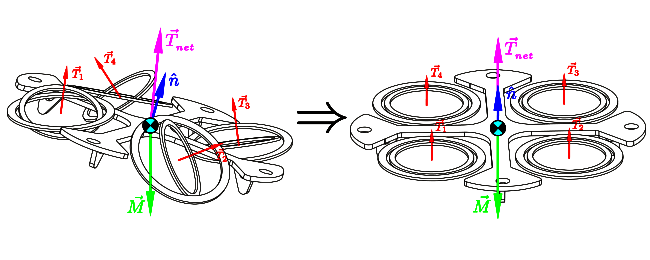
\includegraphics[width=\textwidth]{figs/hover-inertial}
\caption{Hover conditions W.R.T the inertial frame $\mathcal{F}^I$}
\label{fig:hover-inertial}
\end{figure}
\par
Alternatively the hover conditions can be defined with respect to the body frame, being a function of the body's attitude.(Fig:\ref{fig:hover-body}). The difference is that the body's preferred actuator positions are dependent on each instantaneous orientation. That attitude stays constant whilst the actuators are redirected to produce inertial hovering conditions; irrespective of the attitude. The preferred hovering conditions are then always dependent on the commanded attitude trajectory.
\begin{equation}\label{eq:hover-body}
\vec{\nu}_b=
\begin{bmatrix}
\vec{F}_p\hspace{3pt}\\
\vec{\tau}_p\hspace{3pt}
\end{bmatrix}
=\begin{bmatrix}
Q_b^*\otimes\vec{M}\otimes Q_b\\
\vec{0}
\end{bmatrix}~~~~\in\mathcal{F}^b
\end{equation}
\par
\begin{figure}[htbp]
\vspace{-12pt}
\centering
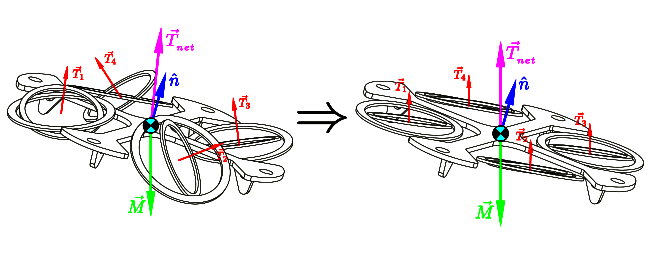
\includegraphics[width=\textwidth]{figs/hover-body}
\vspace{-12pt}
\caption{Hover conditions W.R.T the body frame $\mathcal{F}^b$}
\label{fig:hover-body}
\vspace{-8pt}
\end{figure}
\par
Specific actuator positions are then solved for Eq:\ref{eq:hover} and Eq:\ref{eq:hover-body} using pseudo inversion from Eq:\ref{eq:pseudo-inversion}. The two solutions are then as follows:
\begin{subequations}\label{eq:priority-norm}
\begin{equation}\label{eq:priority-norm-inertial}
u_p^I=R^\dagger(\mathbf{x},\big(B^\dagger(\mathbf{x},\vec{\nu}_I,t)\big),t)
\end{equation}
\vspace{-15pt}
\begin{equation}\label{eq:priority-norm-body}
u_p^b=R^\dagger(\mathbf{x},\big(B^\dagger(\mathbf{x},\vec{\nu}_b,t)\big),t)
\end{equation}
\end{subequations}
Where the inverse rotation operator, $R^\dagger$ from Eq:\ref{eq:priority-norm}, is applied to all four thrust vectors produced by the allocation operator $B^\dagger$. Both actuator matrices are then applied to Eq:\ref{eq:inversion} and could be combined with a non-diagonal weighting matrix.
\begin{subequations}
\begin{equation}
\underset{\in\mathbb{U}}{u}=(\mathbb{I}_{m\times m}-CB(\vec{\mathbf{x}},t)\big)u_p+C\vec{\nu}_d
\end{equation}
\vspace{-10pt}
\begin{equation}
C=W^{-1}B^T(\vec{\mathbf{x}},t)\big(B(\vec{\mathbf{x}},t)W^{-1}B^T(\vec{\mathbf{x}},t)\big)^{-1}
\end{equation}
\end{subequations}
The physical consequences of either preferred actuator positions are demonstrated in simulation in Sec:\ref{subsec:simulation.comparison.allocator}. Priority actuator positions aren't simulated together with weighting matrices, the two are compared independently\ldots
%====================================================
\subsection{Weighted Pseudo Inverse Allocator}
\label{subsec:allocation.allocators.weightedinverse}
%====================================================
Adding weights to the inversion in Eq:\ref{eq:inversion} but regarding preferred actuator positions as negligible, or that $u_p=\vec{0}$, produces a \emph{weighted pseudo inverse} allocator. The positive symmetrical weighting matrix is square with respect to the actuator dimension; here $W\in\mathbb{R}^{12\times 12}$, but more generally $W\in\mathbb{R}^{m\times m}$. The Moore-Penrose inversion (Eq:\ref{eq:pseudo-inversion}) assumes that each actuator is weighted equally. Such a case makes the weighting matrix $W$ purely diagonal; $W\triangleq\mathbb{I}_{m\times m}$. 
\par
A weighting matrix could adapt from time or state dependency following control faults or actuator deterioration. The control objective of a weighted inversion is to design the explicit weighting coefficients as per some preferred heuristic or optimization. Adaptive weighting is not considered or discussed as that is out of the scope for this work and pertains more to FTC\cite{FTCallocation}.
\par
Each weighting coefficient determines how the least squares solution to Eq:\ref{eq:allocation-problem} preferentially biases a particular actuator, in this case the weighting matrix's divisions correlate to mixed actuator thrust vector values. The $3\times 3$ diagonal groupings $W_{1\rightarrow 4}$ relate to individual thrust component biasing ($T_{ix},T_{iy},T_{iz}$) whilst off-centre $3\times 3$ groupings mix separate thrust terms $\vec{T}_{1\rightarrow 4}$. 
\par
Pseudo-inversion, previously, will exactly match the virtual control input $\vec{\nu}_d=B(\mathbf{x},u,t)=\vec{\nu}_c$ so long as the actuators are not saturated. Biasing actuators with different weights could otherwise result in slack between the desired control requirements and their commanded counterparts. Such a case could result in instability given that trajectory tracking is stabilized through Lyapunov's theorem in the design of $\vec{\nu}_d$; not solving for allocated actuator positions. Short of iteratively processing variable weights until a viable solution is found, a constraint on the nature of the weighting matrix needs to be introduced. Online iterative solutions are avoided given their increased computational complexity and the possibility that, given an infinite processing time, a solution may not necessarily be found.
\begin{figure}[htbp]
\centering
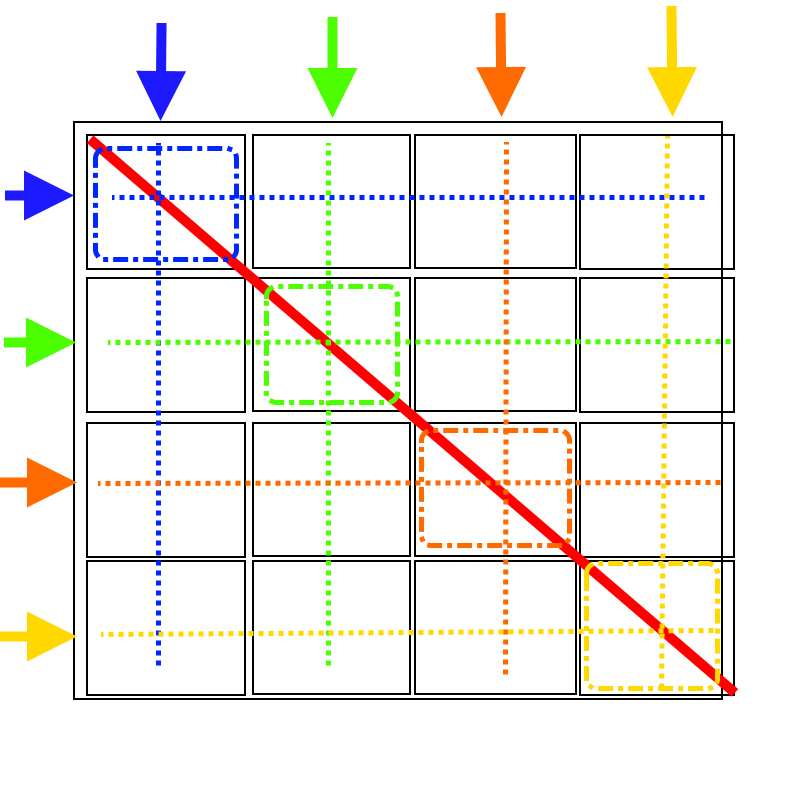
\includegraphics[width=0.6\textwidth]{figs/weighted-matrix}
\label{fig:weighted-matrix}
\caption{Weighting matrix biasing}
\end{figure}
\par
So long each horizontal and vertical weighting groups contributing to each thrust vector, $W_{T_i}\in\mathbb{R}^{3\times 12}$, each have a unit norm, the designed control torque and force inputs will be met. Physically the resultant thrusts and torque (thrust differentials) would be balanced amongst similarly directed components. Furthermore, an additional restraint is that only permissible thrust vector mixings are between opposing pairs; $\vec{T}_1\text{\&}\vec{T}_3$ and $\vec{T}_2\text{\&}\vec{T}_4$. Such a constraint simplifies the time spent optimizing weighting coefficients in Sec:\ref{sec:simulation.allocator}.
\par
The physical consequences of giving priority biasing to thrust vector components in the $\hat{X}_b$ \& $\hat{Y}_b$\footnote{Recalling that the allocator block designs $\vec{T}_{1\rightarrow 4}$ in the body frame, $\in\mathcal{F}^b$. Then the rotation inversion block $R^\dagger(\mathbf{x},\vec{T}_i,t)$ from Eq:\ref{eq:allocator-inersion} finds $(\Omega_i,\lambda_i,\alpha_i)$ to transform $\vec{T}(\Omega_i)$ to the body frame; effectively mapping $\mathcal{F}^{M_i}\rightarrow\mathcal{F}^b$.} directions is that the allocation block prioritizes using pitch or roll servos, $\lambda_i$ \& $\alpha_i$ respectively, before changing the propeller's rotational speed $\Omega_i$. Similarly balancing the of off-diagonal thrust vector mixing blends controller effort amongst opposing actuators. 
\par
The explicit weighting coefficients are to be optimized iteratively in simulation, Sec:\ref{sec:simulation.allocator}; aiming to minimize some performance metric. That metric, which evaluates relative performance of a proposed set of weighting coefficients, is penalized\footnote{More on simulations and optimizations next in Chapter:\ref{ch:simulation}-Simulations \& Results.} from actuator slew rate times and a slack variable norm;
\begin{equation}\label{eq:actuator-penalty}
\int \big(a\norm{t^{\nu_d-\nu_c}-1}+b\norm{s}\big).dt
\end{equation}
Where the integral is run until $t\rightarrow\infty$ over the length of a single simulation cycle. As such, the weighting matrix coefficients try to reduce the transient time taken for the actuator block to settle whilst ensuring stability isn't compromised. Optimization iterations for the weight coefficients are completely independent from the controller coefficient loops to be run in Sec:\ref{sec:simulation.tuning}\ldots
%====================================================
\subsection{Non-linear Plant Control Allocation}
\label{subsec:control.allocation.nonlinear}
%====================================================
\textbf{Come back to this}
\par
Despite the added actuation, each complex dynamic response from an actuator excitation is not fully explotited. The dynamics of an actuator's motor module, Sec:\ref{subsec:dynamics.nonlinearities.gyrotorques}, until now has been treated as an element to be compensated for in feedback structure. An alternative approach, seen in Gasco, et al. [2012]\cite{tiltgasco,tiltrihani}, is to use the actuator reactions as additional non-linear actuator plants. In \cite{tiltgasco,tiltrihani} the actuator plants and their resultant dynamics were introduced as additional dimensions to the actuator matrix $u\in\mathbb{U}$. 
\par
Such an approach was achievable because the authors, despite adding two extra degrees of freedom for each propeller, hadn't vectored the propeller thrust. The non-linear proposal here is to first calculate a Pseudo-inversion actuator solution \emph{without} plant compensation\footnote{Disregarding $\vec{\tau}_Q,\vec{\tau}_g$ \& $\vec{Q}$.}, then introducing those induced actuator responses from such an excitation to alleviate the control plant requirement. A subsequent revised virtual control plant input is used iteratively to find a subsequent pseudo-inversion solution; the process is cycled until the control requirements are met.
\par
\begin{figure}[hbtp]
\centering
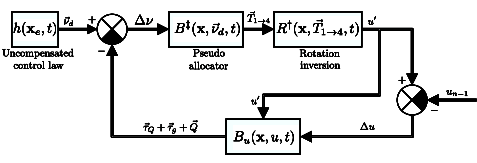
\includegraphics[width=0.6\textwidth]{figs/allocation}
\caption{Allocation loop iteration}
\label{fig:non-linear-allocation}
\end{figure}
In Fig:\ref{fig:non-linear-allocation} the iteration loop is shown, each iteration is run online and settles at a balance point. In the loop, the block $B_u(\mathbf{x},u,t)$ is a combination of non-linear actuator response terms from Eq:\ref{eq:actuator-torque},\ref{eq:grav-torque} \& \ref{eq:aerodynamic-torque}; those being $\vec{\tau}_Q$, $\vec{\tau}_g$ \& $\vec{Q}$ respectively. The settling point, where possible, a portion of the commanded control input $\vec{\nu}_d$ is achieved from the otherwise compensated for actuator response dynamics.